\documentclass[../../Installationguide_Unity_Pupil]{subfiles}
% Hier müssen keine Packages geladen werden, es werden automatisch die von masterdoc geladen,
% sowie die Konfigurationen.
% Bei includegraphics nur Bildname (Bsp: Bild.png) eingeben, da er in den angegebenen Pfade die Bilder sucht
\graphicspath{{img/}{../../img/}}

\begin{document}

\chapter{Installation of Pupil Capture}
Estimated time for installation: 30 minutes\\
$~$\\
Pupil Capture is an eye tracking software by Pupil Labs and is used by our framework. It's open source and you can easily expand it with own plugins. \\
This chapter describes all the steps for installing the PyUVC driver on Windows, which is neccessary to use a camera for Pupil Capture.
Before the plugin can be initialized, please refer to \href{https://github.com/pupil-labs/pupil/releases }{this webpage} to find the correct version which matches your OS. Preferably v0.9.12.
\section{PyUVC driver installation for  Pupil Capture}
\begin{enumerate}
	\item Download and install the driver \href{https://sourceforge.net/projects/libusbk/files/libusbK-release/3.0.7.0/libusbK-3.0.7.0-setup.exe/download}{libusbk 3.0.7.0}.
	\item Next download \href{http://zadig.akeo.ie/downloads/zadig_2.2.exe}{Zadig}.
	\item Connect your camera with the computer.
	\item Run Zadig and open Options. You can see all currently selected option. Select and deselect the options according to figure \ref{fig:Options}.
	\begin{figure}[htb]
		\centering
		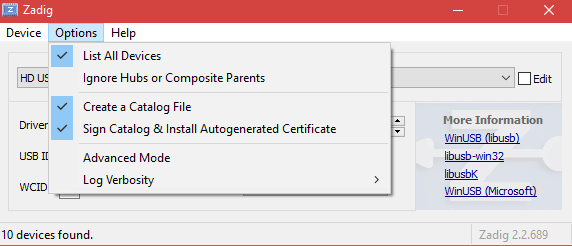
\includegraphics[width=\textwidth]{img/Zadiq_Options.png}
		\caption{Selected options}
		\label{fig:Options}
	\end{figure}
	\item Now you should see a list of all connected USB devices. Select your device, which is marked with the addition 'composite parent'. A possible selection is shown on the figure \ref{fig:Composite}.
	\begin{figure}[htb]
		\centering
		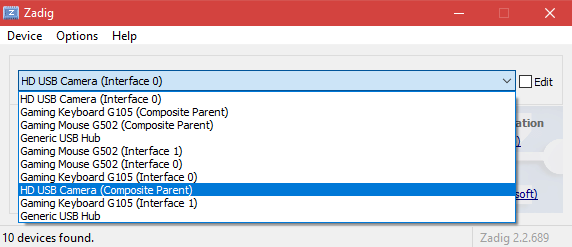
\includegraphics[width=\textwidth]{img/Zadiq_Composite_Parent.png}
		\caption{Example USB camera}
		\label{fig:Composite}
	\end{figure}
	\item Set the driver of your device on 'libusbK (v3.0.7.0)' and press 'replace driver' (Fig. \ref{fig:Driver})
	\begin{figure}[htb]
		\centering
		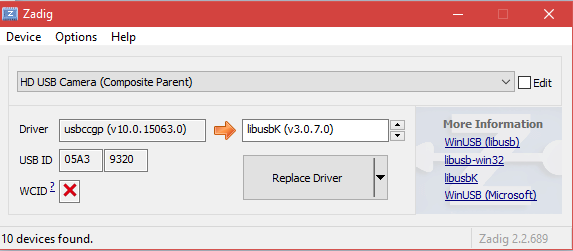
\includegraphics[width=\textwidth]{img/Zadiq_libusbK.png}
		\caption{Driver selection}
		\label{fig:Driver}
	\end{figure}
	\item Start Pupil Capture and verify that the driver installation was successful by selecting the camera as the USB device. If this is not the case, please run the driver installation again.
\end{enumerate}
\clearpage

\section{Plug-In Integration}
Once the Pupil Capture software and the drivers are installed, the last step will be integrating our plugin for video streaming. Just follow these few steps:
\begin{enumerate}
	\item If you haven’t done it yet, run Pupil Capture once. This should create a directory called ``pupil\_capture\_settings'' in your home directory e.g. $<root>/Users/<username>$ (Windows), $/Users/<username>$ (Mac).
	\item Locate the directory called ``plugins'' in this folder and drop our python file ``unity\_streaming\_plugin'' here. 	
	\item After restarting Pupil Capture the software should load the plugin automatically, and an additional capture source for streaming video data from an Unity application should appear in the capture selection selector in the world window. 
\end{enumerate}

\end{document}